%===================================================================================
% JORNADA CIENTÍFICA ESTUDIANTIL - MATCOM, UH
%===================================================================================
% Esta plantilla ha sido diseñada para ser usada en los artículos de la
% Jornada Científica Estudiantil, MatCom.
%
% Por favor, siga las instrucciones de esta plantilla y rellene en las secciones
% correspondientes.
%
% NOTA: Necesitará el archivo 'jcematcom.sty' en la misma carpeta donde esté este
%       archivo para poder utilizar esta plantila.
%===================================================================================



%===================================================================================
% PREÁMBULO
%-----------------------------------------------------------------------------------
\documentclass[a4paper,10pt,twocolumn]{article}

%===================================================================================
% Paquetes
%-----------------------------------------------------------------------------------
\usepackage{amsmath}
\usepackage{amsfonts}
\usepackage{amssymb}
\usepackage{jcematcom}
\usepackage[utf8]{inputenc}
\usepackage[spanish]{babel}
\usepackage{listings}
\usepackage[pdftex]{hyperref}
\usepackage{graphicx}
%-----------------------------------------------------------------------------------
% Configuración
%-----------------------------------------------------------------------------------
\hypersetup{colorlinks,%
	    citecolor=black,%
	    filecolor=black,%
	    linkcolor=black,%
	    urlcolor=blue}

\graphicspath{ {./images/} }
%===================================================================================



%===================================================================================
% Presentacion
%-----------------------------------------------------------------------------------
% Título
%-----------------------------------------------------------------------------------
\title{Estadística\\Proyecto Fase 2}

%-----------------------------------------------------------------------------------
% Autores
%-----------------------------------------------------------------------------------
\author{\\
\name Carlos Bermudez Porto \email \href{mailto:c.bermudez@estudiantes.matcom.uh.cu}{c.bermudez@estudiantes.matcom.uh.cu}
	\\ \addr Grupo C412 \AND
\name Leynier Gutiérrez González \email \href{mailto:l.gutierrez@estudiantes.matcom.uh.cu}{l.gutierrez@estudiantes.matcom.uh.cu}
  \\ \addr Grupo C412 \AND
\name Tony Raúl Blanco Fernández \email \href{mailto:t.blanco@estudiantes.matcom.uh.cu}{t.blanco@estudiantes.matcom.uh.cu}
  \\ \addr Grupo C411}

%-----------------------------------------------------------------------------------
% Tutores
%-----------------------------------------------------------------------------------
\tutors{\\
Lic. Dalia Diaz Sistachs, \emph{Departamento de Matemática Aplicada}}

%-----------------------------------------------------------------------------------
% Headings
%-----------------------------------------------------------------------------------
\jcematcomheading{\the\year}{1-\pageref{end}}{C. Bermudez, L. Gutiérrez, T. Blanco}

%-----------------------------------------------------------------------------------
\ShortHeadings{Proyecto Fase 2 de Estadística}{Autores}
%===================================================================================

\hyphenation{se-leccio-na-das va-ria-ble res-pues-ta pre-sen-cia in-de-pen-dien-tes Re-si-duos erro-res va-rian-za}

%===================================================================================
% DOCUMENTO
%-----------------------------------------------------------------------------------
\begin{document}

%-----------------------------------------------------------------------------------
% NO BORRAR ESTA LINEA!
%-----------------------------------------------------------------------------------
\twocolumn[
%-----------------------------------------------------------------------------------

\maketitle

%===================================================================================
% Resumen y Abstract
%-----------------------------------------------------------------------------------
\selectlanguage{spanish} % Para producir el documento en Español

%-----------------------------------------------------------------------------------
% Resumen en Español
%-----------------------------------------------------------------------------------
% \begin{abstract}

% 	El Resumen en Español debe constar de $100$ a $200$ palabras y presentar de forma
% 	clara y concisa el contenido fundamental del artículo.

% \end{abstract}

%-----------------------------------------------------------------------------------
% English Abstract
%-----------------------------------------------------------------------------------
% \vspace{0.5cm}

% \begin{enabstract}

%   The English Abstract must have have $100$ to $200$ words, and present in a clear
%   and concise form the essentials of the article content.

% \end{enabstract}

%-----------------------------------------------------------------------------------
% Palabras clave
%-----------------------------------------------------------------------------------
\begin{keywords}
	Estadística,
	Regresión,
	Lineal,
	Reducción,
	Dimensión,
	ANOVA
\end{keywords}

%-----------------------------------------------------------------------------------
% Temas
%-----------------------------------------------------------------------------------
\begin{topics}
	Estadística, Regresión Lineal, ANOVA.
\end{topics}


%-----------------------------------------------------------------------------------
% NO BORRAR ESTAS LINEAS!
%-----------------------------------------------------------------------------------
\vspace{0.8cm}
]
%-----------------------------------------------------------------------------------


%===================================================================================

%===================================================================================
% Introducción
%-----------------------------------------------------------------------------------
\section{Introducción}\label{sec:intro}
%-----------------------------------------------------------------------------------

El siguiente trabajo corresponde a la investigación de los autores como evaluación de la asignatura de Estadística de la carrera de Ciencia de la Computación de la Facultad de Matemática y Computación de la Universidad de La Habana.

Los datos utilizados para la investigación son sacados de una base de datos del FIFA 15, la cual contiene todos los jugadores existentes en este videojuego, en la que cada jugador tiene varias estadísticas de sus habilidades como valoración general \textit{(overall)}, potencial \textit{(potential)}, entre otras. Además de la nacionalidad, pie preferido, club al que pertenece, etc.

Se decidió analizar el comportamiento de los jugadores de clase mundial, por lo que se redujo el análisis a los jugadores que pertenecen a los equipos de la fase de grupos de la UEFA Champions League de la temporada 2014-2015, ya que en esta competición participan los mejores clubes de futbol de las mejores ligas, considerado la competición de clubes más importante.

En las pruebas de hipótesis se asumió un nivel de significación del $5\%$, por tanto, fue posible aceptar las hipótesis nulas con una probabilidad de error menor o igual a $0.05$.

\subsection{Selección y descripción general de los datos}\label{sec:sel_desc}

De todas las variables disponibles en la base de datos, se seleccionaron $17$ porque se consideró son las que mejor describen la forma de jugar de un futbolista. Estas son:

\begin{itemize}
	\item overall
	\item potential
	\item attacking\_finishing
	\item attacking\_short\_passing
	\item skill\_ball\_control
	\item skill\_fk\_accuracy
	\item skill\_long\_passing
	\item movement\_agility
	\item movement\_balance
	\item movement\_sprint\_speed
	\item power\_shot\_power
	\item power\_stamina
	\item power\_long\_shots
	\item mentality\_interceptions
	\item mentality\_vision
	\item defending\_marking
	\item defending\_sliding\_tackle
\end{itemize}

Se realizó un análisis general de esas variables utilizando la función $skim$ de la biblioteca $skimr$. El resultado se puede ver en la Fig. \ref{fig:skim}.

\begin{figure}[htb]%
	\begin{center}
		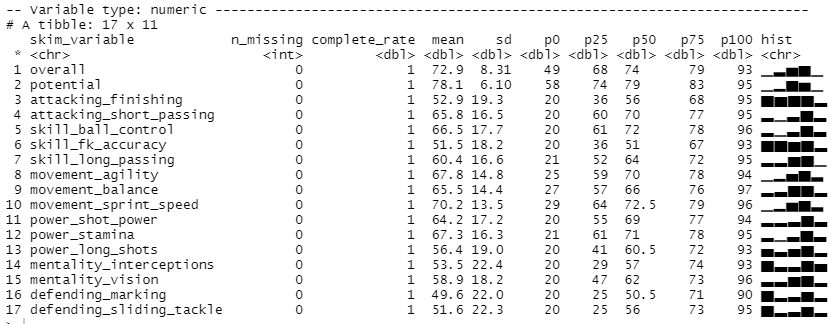
\includegraphics[width=\linewidth]{skim}
	\end{center}
	\caption{Resultado de aplicar la función $skim$ \label{fig:skim}}%
\end{figure}

Como resultado del análisis general se detectó que la media de las habilidades de los jugadores es baja incluso para los mejores equipos de las mejores ligas de futbol. A partir de cálculo de los cuartiles el $75\%$ de los jugadores están por debajo de $80$ puntos (exceptuando el caso del $potential$ que alcanza $83$) lo cual quiere decir que los jugadores considerados clase mundial corresponden solo a un $15\%$.

%===================================================================================


%===================================================================================
% Regresión Lineal y Análisis de Componentes Principales
%-----------------------------------------------------------------------------------
\section{Regresión Lineal y Análisis de Componentes Principales}\label{sec:reg_acp}
%-----------------------------------------------------------------------------------

Para aplicar la regresión es necesario realizar un análisis de las correlaciones de las variables seleccionadas.

\begin{figure}[htb]%
	\begin{center}
		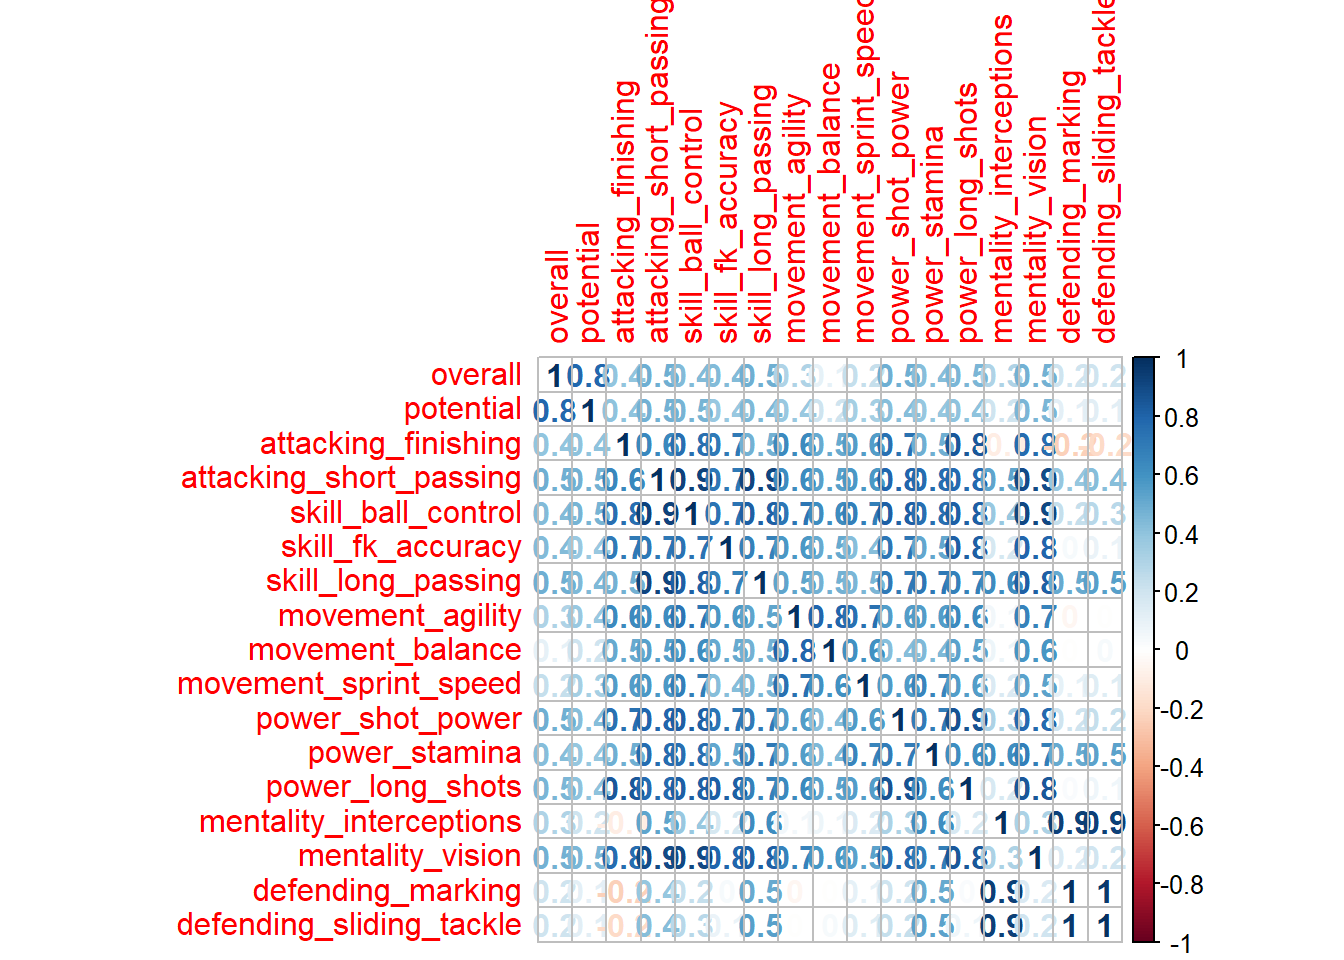
\includegraphics[width=\linewidth]{cor_general}
	\end{center}
	\caption{Correlación de todas las variables \label{fig:cor_general}}%
\end{figure}

Como resultado del análisis de la Fig. \ref{fig:cor_general}, se detectó una alta correlación entre las variables, por lo que no sería correcto aplicar una regresión lineal, por lo tanto, se aplicó la técnica de reducción de dimensiones para obtener las componentes principales que sean independientes entre sí y que sean dependientes de una variable respuesta elegida.

\subsection{Análisis de Componentes Principales}\label{sec:acp}

En un inicio se seleccionó como variable respuesta a $overall$, por lo que se hizo necesario extraer esa variable antes de realizar el análisis de las componentes principales.

\begin{figure}[htb]%
	\begin{center}
		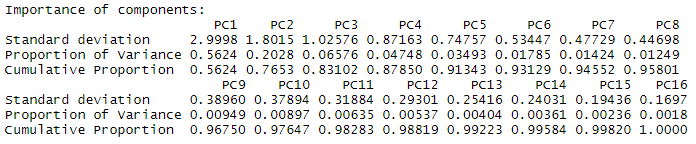
\includegraphics[width=\linewidth]{acp_sum}
	\end{center}
	\caption{Análisis de Componentes Principales \label{fig:acp_sum}}%
\end{figure}

Aplicando el criterio de \textit{Kaiser}, fue posible quedarse con las primeras tres componentes. Pasando a crear una matriz con la variable respuesta junta las tres componentes principales seleccionadas y analizando sus correlaciones.

\begin{figure}[htb]%
	\begin{center}
		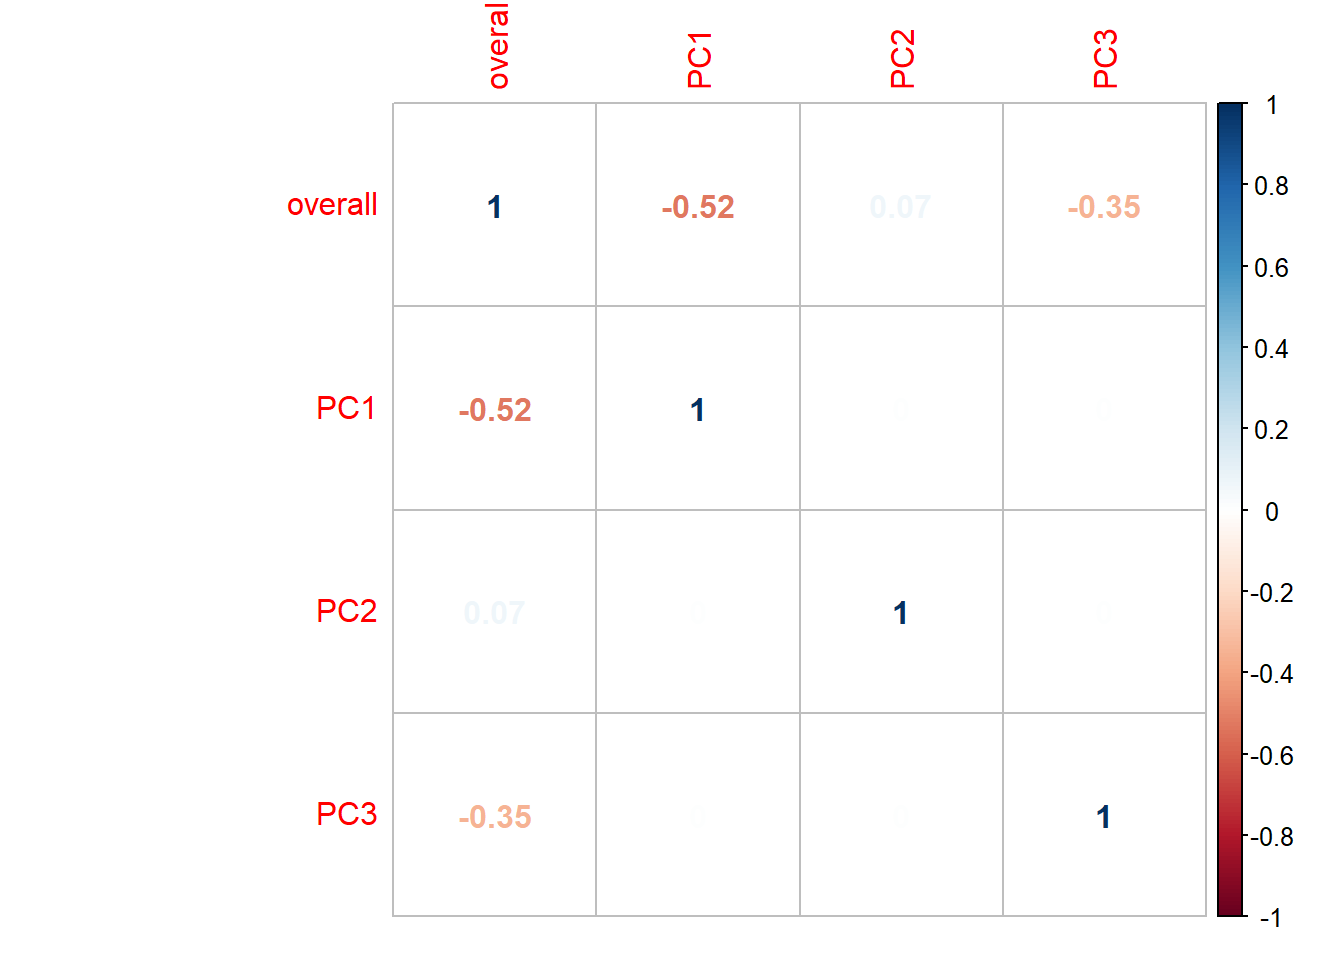
\includegraphics[width=\linewidth]{cor_acp_1}
	\end{center}
	\caption{Correlación 1 de las Componentes Principales \label{fig:cor_acp_1}}%
\end{figure}

Como se puede ver en la Fig. \ref{fig:cor_acp_1} la variable respuesta escogida no tiene dependencia con las componentes principales seleccionadas, luego se realizó un análisis similar iterando por todas las variables seleccionándolas como variable respuesta en cada paso se obtiene que la variable $mentality\_interceptions$ tiene una mayor correlación con las componentes principales seleccionadas (referirse a la Fig. \ref{fig:cor_acp_2}) por lo que era una mejor opción a variable respuesta.

\begin{figure}[htb]%
	\begin{center}
		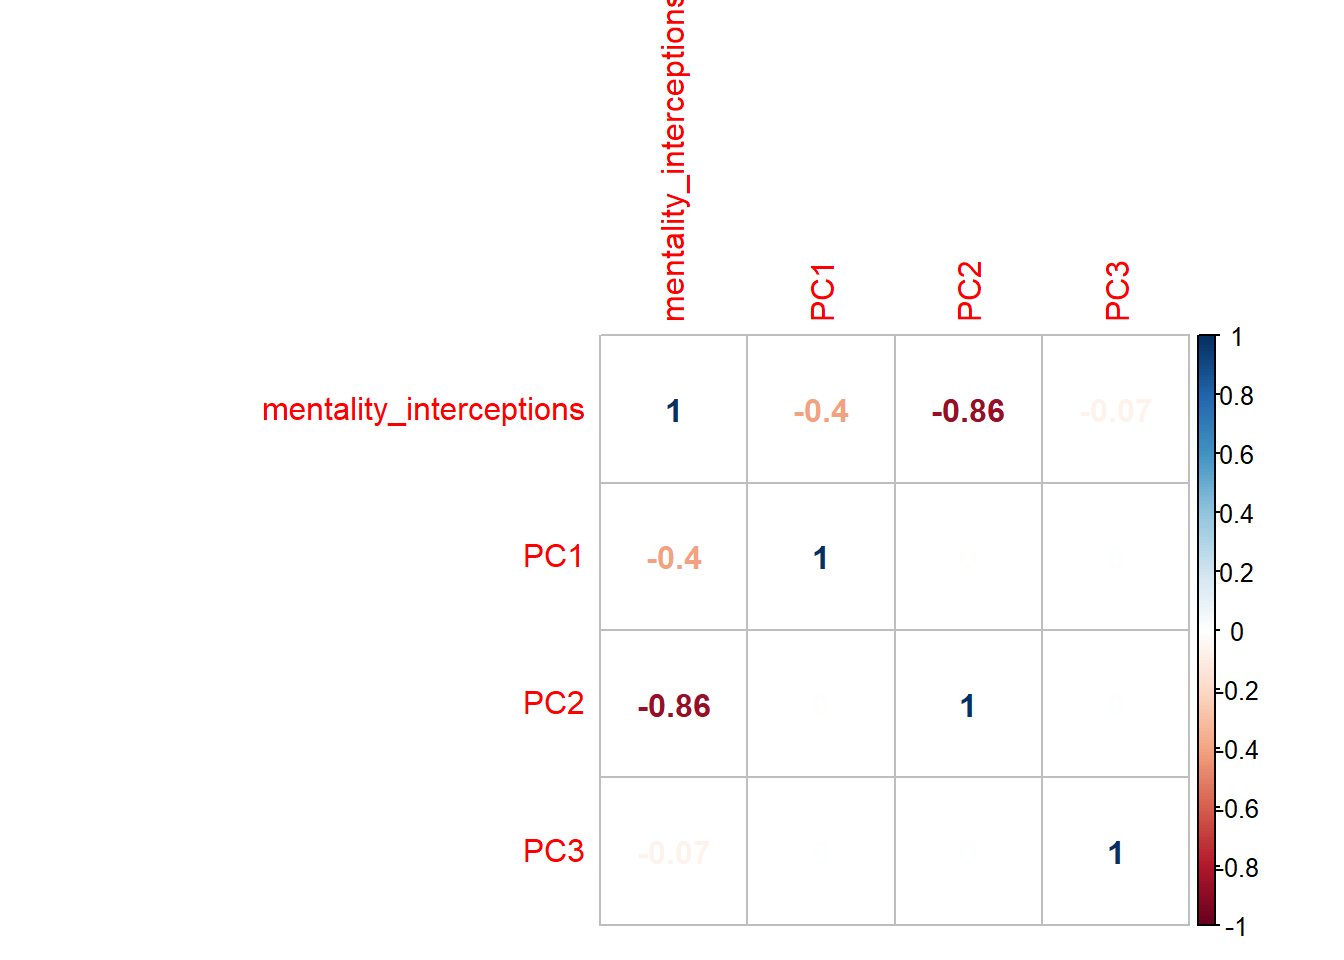
\includegraphics[width=\linewidth]{cor_acp_2}
	\end{center}
	\caption{Correlación 2 de las Componentes Principales \label{fig:cor_acp_2}}%
\end{figure}

\subsubsection{Descripción de las Componentes}\label{sec:desc_comp}

\begin{itemize}
	\item \textbf{PC1:} La componente se caracteriza por una presencia negativa de \textit{overall}, \textit{potential}, \textit{attacking\_finishing}, \textit{attacking\_short\_passing}, \textit{skill\_ball\_control}, \textit{skill\_fk\_accuracy}, \textit{skill\_long\_passing}, \textit{movement\_agility}, \textit{movement\_balance} y \textit{movement\_sprint\_speed}. Se puede interpretar como que son los jugadores no tan habilidosos, los cuales, como vimos en análisis anteriores, son la mayoría.

	\item \textbf{PC2:} La componente se caracteriza por una presencia positiva de \textit{attacking\_finishing} y una presencia negativa de \textit{defending\_marking} y de \textit{defending\_sliding\_tackle}. Se puede interpretar como los jugadores de la posición de delantero centro. Ya que su función es marcar goles y no tienen mucha obligación defensiva.

	\item \textbf{PC3:} La componente se caracteriza por una presencia positiva de \textit{overall} y \textit{potential}, y una presencia negativa de \textit{movement\_balance}. Se puede interpretar como los jugadores habilidosos pero con tendencia a caer mucho en el campo, ya sea por excesiva cantidad de faltas o por engañar al arbitro.
\end{itemize}

\subsection{Regresión Lineal}\label{sec:reg_li}

Teniendo como la variable respuesta a \textit{mentality\_interceptions} y como variables independientes las componentes principales se realizó un modelo de regresión lineal múltiple, a continuación, se muestra la información del modelo realizado.

\begin{figure}[htb]%
	\begin{center}
		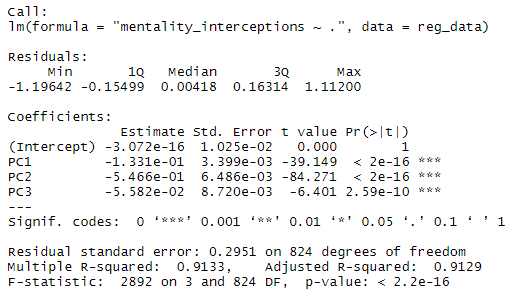
\includegraphics[width=\linewidth]{reg_li}
	\end{center}
	\caption{Resultado del Modelo de Regresión Lineal \label{fig:reg_li}}%
\end{figure}

De la información de la Fig. \ref{fig:reg_li} se deduce la siguiente ecuación para determinar \textit{mentality\_interceptions} en base a las componentes principales.

$$ mentality_{interceptions} = -0.13 PC_1 - 0.55 PC_2 - 0.06 PC_3 $$

Uno de los factores a tener en cuenta es la estandarización de los datos durante el proceso de clasificación, por lo que su efecto se ve reflejado en la ausencia del término independiente en la ecuación de regresión.

La precisión del modelo, medida en términos del valor del $Ajusted\ R-squared$ es de $0.9129$ lo cual es bastante alto tomando en consideración el desprecio de datos resultante del análisis de las componentes principales. El $p-value$ de la prueba de $F-statistic$ es menor que $0.05$ por lo que podemos asegurar que el modelo produce resultados. El error residual es de $0.2951$.

\subsubsection{Análisis de los supuestos}\label{sec:reg_err}

Los supuestos de la regresión linear son los siguientes:

\begin{enumerate}
	\item Las variables independientes no están correlacionadas.
	\item La media y la suma de los errores es cero.
	\item Los errores son independientes.
	\item Los errores tienen distribución normal.
	\item La varianza de los errores es constante.
\end{enumerate}

El \textbf{primer supuesto} se cumple porque las variables independientes utilizadas son resultado del análisis de componentes principales.

El \textbf{segundo supuesto} también se cumple, siendo la media y la suma de los errores extremadamente cercanos a cero. (Fig. \ref{fig:reg_mean_sum})

\begin{figure}[htb]%
	\begin{center}
		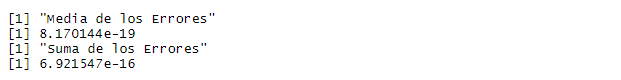
\includegraphics[width=\linewidth]{reg_mean_sum}
	\end{center}
	\caption{Media y suma de los errores \label{fig:reg_mean_sum}}%
\end{figure}

El \textbf{tercer supuesto}, que los errores sean independientes, como se puede ver la prueba de \textit{Durbin-Watson} no es significativa, siendo el $p-value$ mayor que $0.05$, no se puede rechazar la hipótesis nula, por tanto, se puede deducir que los errores son independientes entre sí. (Fig. \ref{fig:reg_dwtest})

\begin{figure}[htb]%
	\begin{center}
		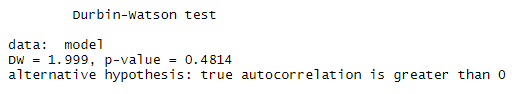
\includegraphics[width=\linewidth]{reg_dwtest}
	\end{center}
	\caption{Prueba de Durbin-Watson \label{fig:reg_dwtest}}%
\end{figure}

El \textbf{cuarto supuesto}, que los errores tengan una distribución normal, se analizó en primera instancia el histograma de los errores (Fig. \ref{fig:reg_his}) y el Q-Q Plot (Fig. \ref{fig:reg_qq}).

\begin{figure}[htb]%
	\begin{center}
		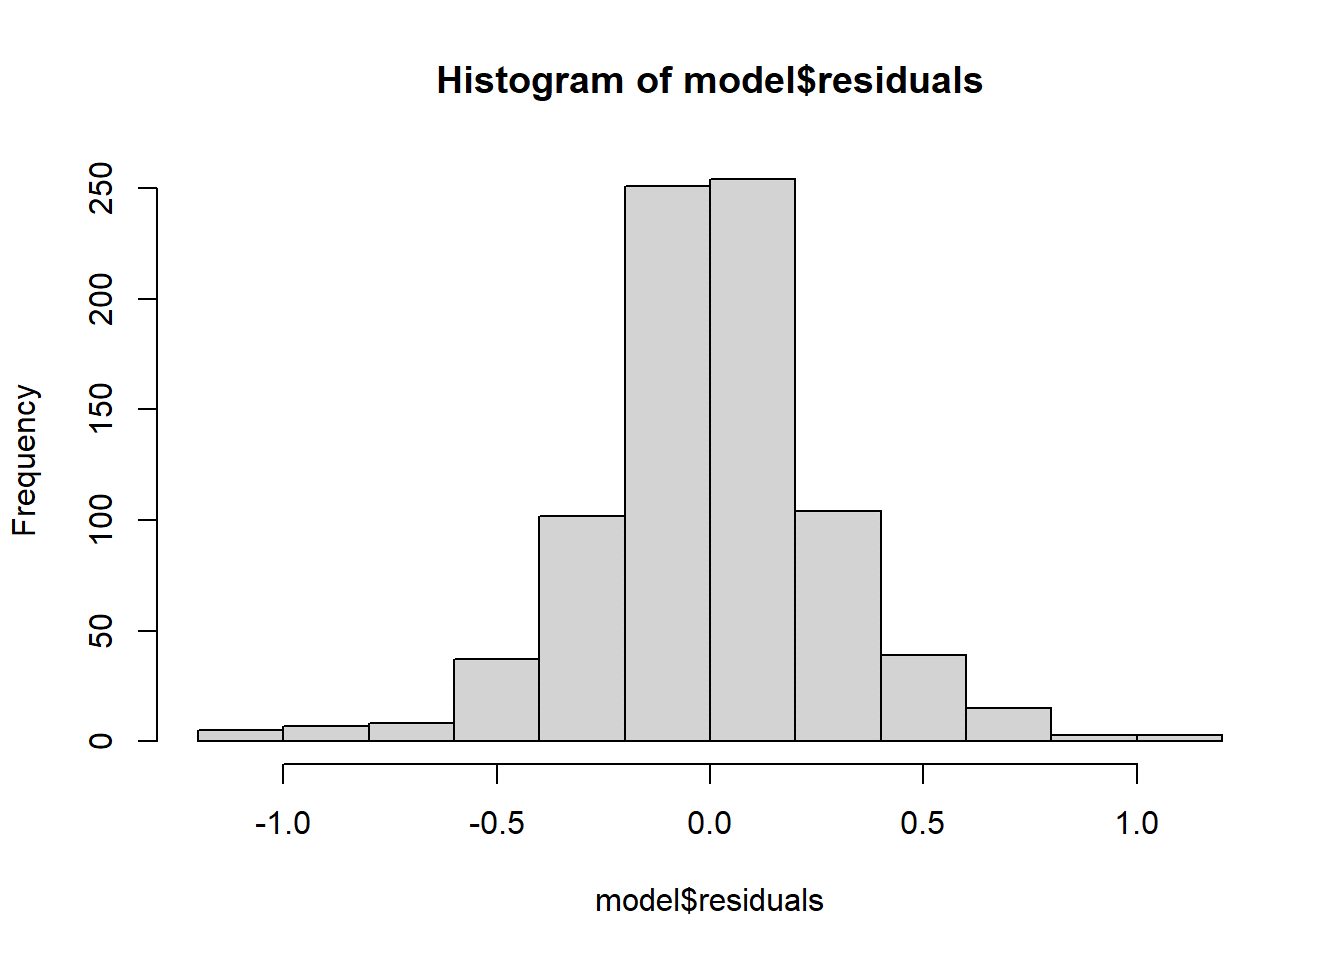
\includegraphics[width=\linewidth]{reg_his}
	\end{center}
	\caption{Histograma de los errores \label{fig:reg_his}}%
\end{figure}

\begin{figure}[htb]%
	\begin{center}
		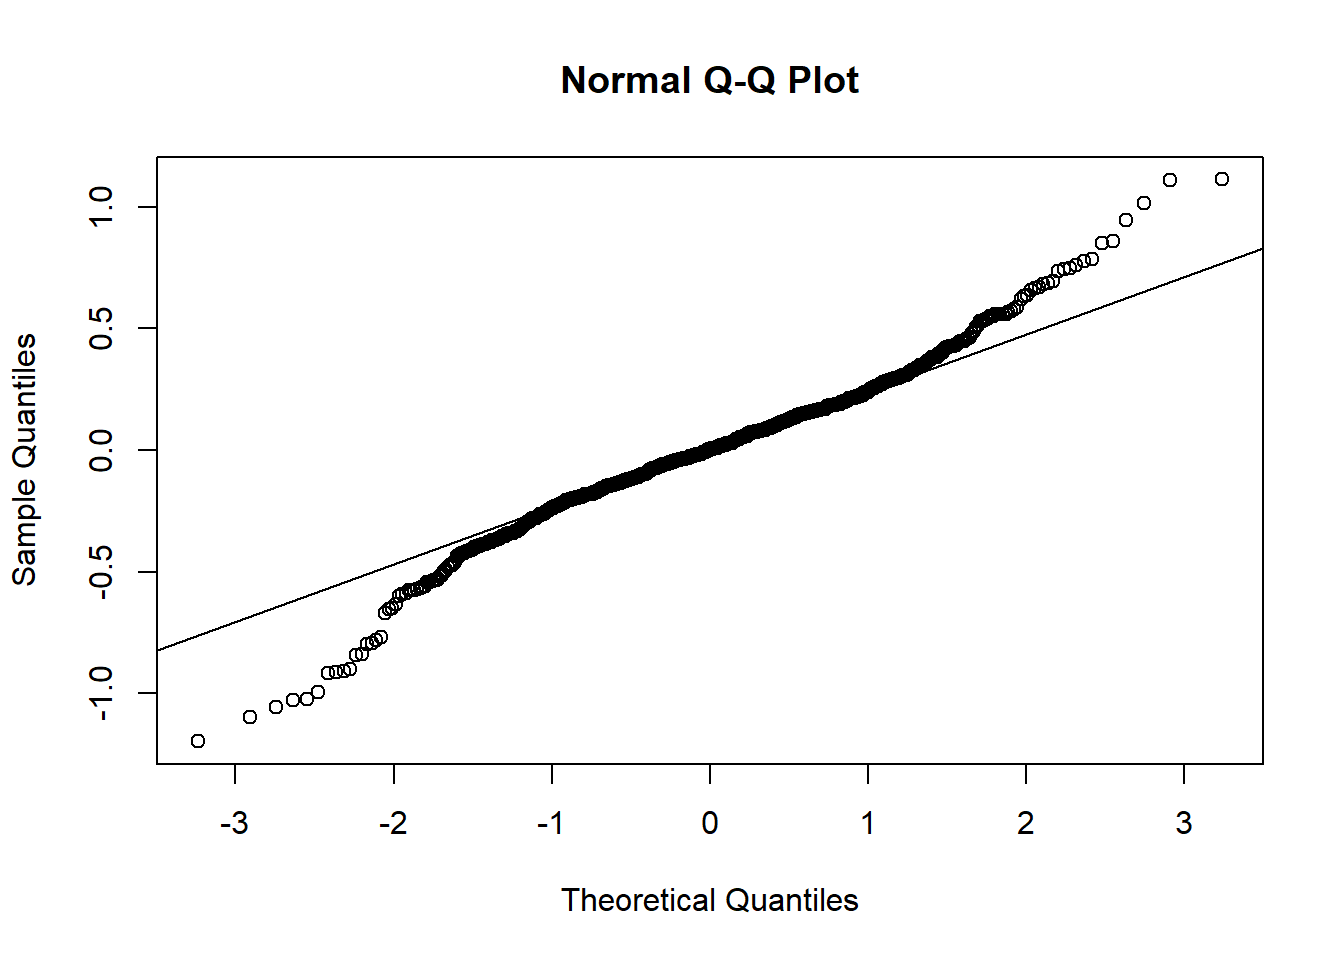
\includegraphics[width=\linewidth]{reg_qq}
	\end{center}
	\caption{QQ-Plot de los errores \label{fig:reg_qq}}%
\end{figure}

\begin{figure}[htb]%
	\begin{center}
		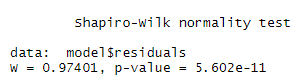
\includegraphics[width=\linewidth]{reg_shapiro}
	\end{center}
	\caption{Prueba de Shapiro-Wilk \label{fig:reg_shapiro}}%
\end{figure}

A partir de la interpretación del histograma (Fig. \ref{fig:reg_his}) se pudo observar una distribución normal, pero no tanto a partir de la interpretación del Q-Q Plot (Fig. \ref{fig:reg_qq}), por lo que se realizó una prueba de $Shapiro-Wilk$ (Fig. \ref{fig:reg_shapiro}).

Como se puede ver la prueba de $Shapiro-Wilk$ (Fig. \ref{fig:reg_shapiro}) es significativa, siendo el $p-value$ menor que $0.05$, se puede rechazar la hipótesis nula, por tanto, se puede deducir que los errores no siguen una distribución normal, incumpliendo con los supuestos, y, por tanto, el modelo no es de utilidad.

Al incumplirse uno de los supuestos, el modelo deja de tener utilidad, pero aun así, se decidió analizar la homocedasticidad en este trabajo.

El \textbf{quito supuesto}, que la varianza de los errores se constante, se analizó en primera instancia el gráfico de los Residuos Estandarizados (Fig. \ref{fig:reg_res}).

\begin{figure}[htb]%
	\begin{center}
		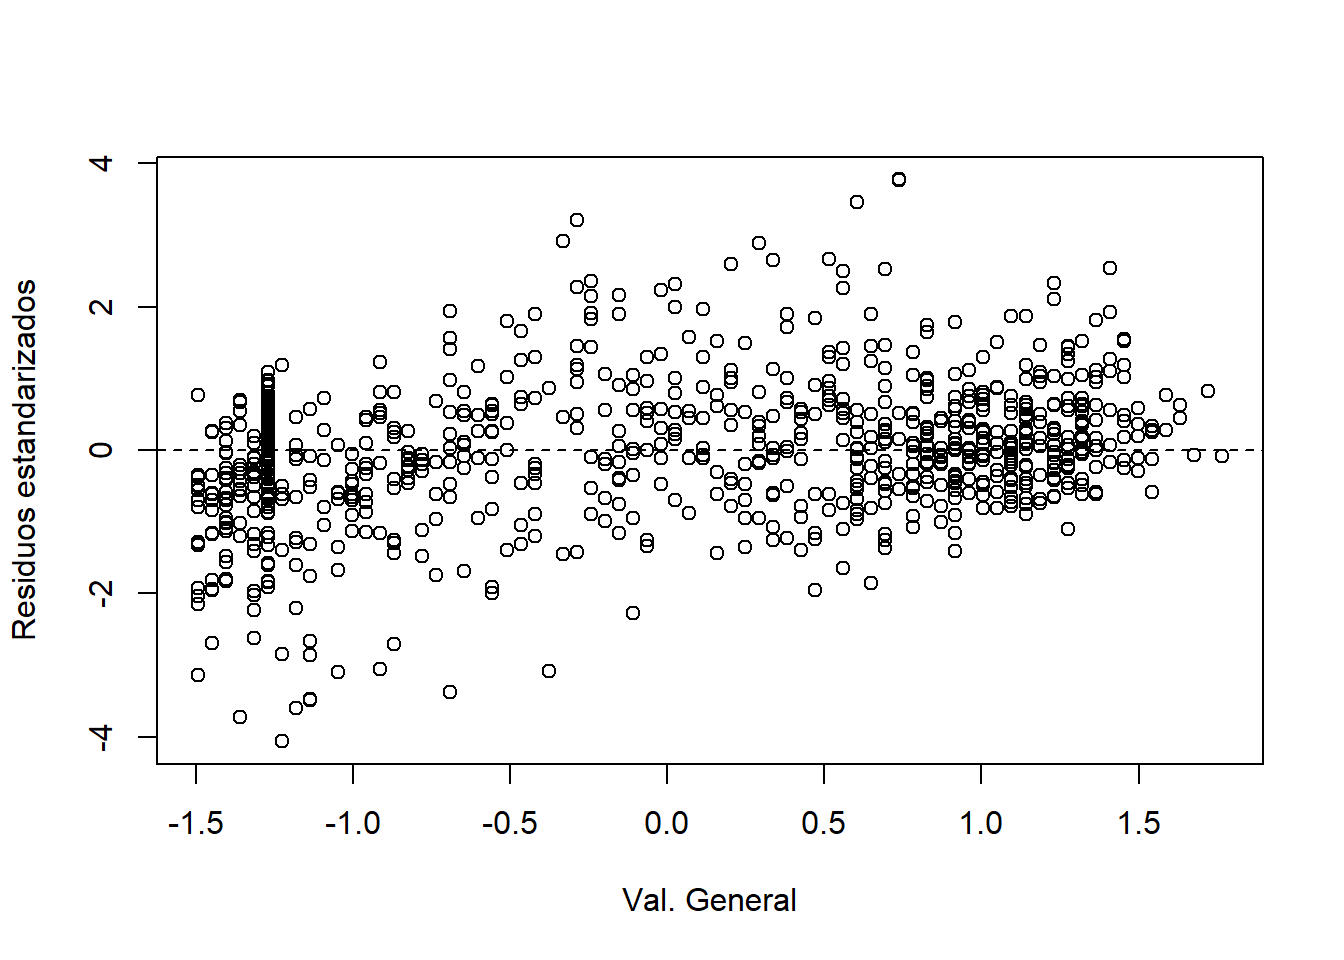
\includegraphics[width=\linewidth]{reg_res}
	\end{center}
	\caption{Residuos Estandarizados \label{fig:reg_res}}%
\end{figure}

A partir de la interpretación del gráfico de los Residuos Estandarizados (Fig. \ref{fig:reg_res}) se pudo observar una homocedasticidad en los errores, pero no quedó muy claro, por lo que se realizó una prueba de $Breushc-Pagan$ (Fig. \ref{fig:reg_bptest}) para confirmarlo.

\begin{figure}[htb]%
	\begin{center}
		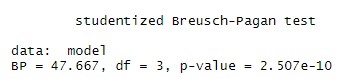
\includegraphics[width=\linewidth]{reg_bptest}
	\end{center}
	\caption{Prueba de Breushc-Pagan \label{fig:reg_bptest}}%
\end{figure}

Como se pudo ver, la prueba de $Breushc-Pagan$ (Fig. \ref{fig:reg_bptest}) es significativa, siendo el $p-value$ menor que $0.05$, se pudo rechazar la hipótesis nula, por tanto, se pudo deducir que no hay heteroscedasticidad en los errores (de donde se dedujo que hay homocedasticidad)

\section{ANOVA}\label{sec:anova}

Para el ANOVA o análisis de varianzas se decidió analizar si el pie preferido influye en la habilidad de deslizarse de los jugadores. A continuación se muestra el resultado del modelo (Fig. \ref{fig:anova_sum}).

\begin{figure}[htb]%
	\begin{center}
		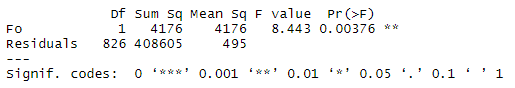
\includegraphics[width=\linewidth]{anova_sum}
	\end{center}
	\caption{Resultado de ANOVA \label{fig:anova_sum}}%
\end{figure}

Como el $p-value$ es menor que la significación prefijada de $0.05$, se rechaza la hipótesis nula y se acepta que el pie preferido influye en la habilidad para deslizarse.

\subsection{Análisis de los supuestos}\label{sec:anova_sup}

\begin{enumerate}
	\item Los errores siguen una distribución normal con media cero.
	\item Los errores son independientes entre sí.
	\item Los errores tienen la misma varianza.
\end{enumerate}

El \textbf{primer supuesto}, que los errores tengan una distribución normal con media cero, se analizó en primera instancia el histograma de los errores (Fig. \ref{fig:anova_his}) y el Q-Q Plot (Fig. \ref{fig:anova_qq}).

\begin{figure}[htb]%
	\begin{center}
		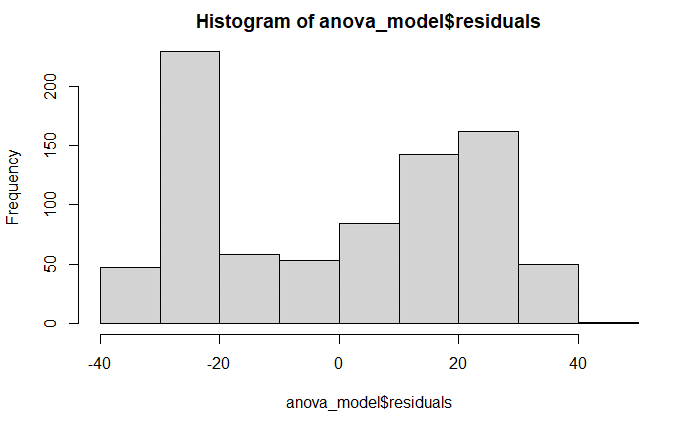
\includegraphics[width=\linewidth]{anova_his}
	\end{center}
	\caption{Histograma de los errores del modelo de ANOVA \label{fig:anova_his}}%
\end{figure}

\begin{figure}[htb]%
	\begin{center}
		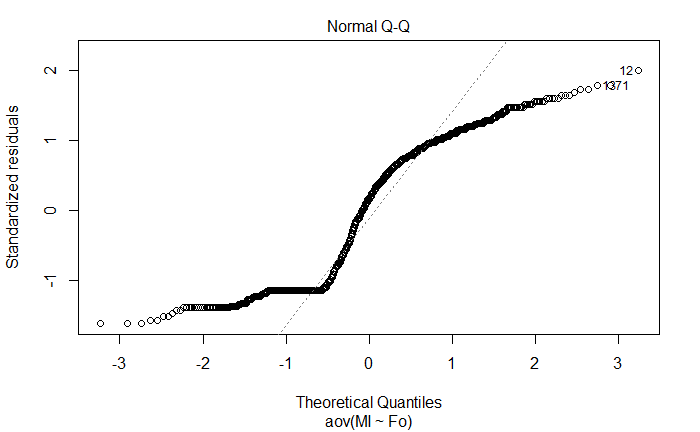
\includegraphics[width=\linewidth]{anova_qq}
	\end{center}
	\caption{Q-Q Plot del modelo de ANOVA \label{fig:anova_qq}}%
\end{figure}

A partir de la interpretación del histograma (Fig. \ref{fig:anova_his}) y del Q-Q Plot (Fig. \ref{fig:anova_qq}) se pudo observar que la distribución no es normal, por lo que se realizó una prueba de $Shapiro-Wilk$ (Fig. \ref{fig:anova_shapiro}) para confírmalo.

\begin{figure}[htb]%
	\begin{center}
		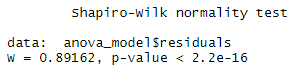
\includegraphics[width=\linewidth]{anova_shapiro}
	\end{center}
	\caption{Prueba de Shapiro-Wilk \label{fig:anova_shapiro}}%
\end{figure}

Como se puede ver la prueba de $Shapiro-Wilk$ (Fig. \ref{fig:anova_shapiro}) es significativa, siendo el $p-value$ menor que $0.05$, se puede rechazar la hipótesis nula, por tanto, se puede deducir que los errores no siguen una distribución normal, incumpliendo con los supuestos, y, por tanto, el modelo no es de utilidad.

Al incumplirse uno de los supuestos, el modelo deja de tener utilidad, pero, aun así, se decidió verificar los restantes supuestos.

El \textbf{segundo supuesto}, que los errores sean independientes entre sí, como se puede ver la prueba de $Durbin-Watson$ (Fig. \ref{fig:anova_dwtest}) es significativa, siendo el $p-value$ menor que $0.05$, se puede rechazar la hipótesis nula, por tanto, se puede deducir que los errores no son independientes entre sí, incumpliendo con los supuestos, y, por tanto, el modelo no es de utilidad.

\begin{figure}[htb]%
	\begin{center}
		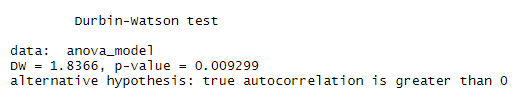
\includegraphics[width=\linewidth]{anova_dwtest}
	\end{center}
	\caption{Prueba de Durbin-Watson \label{fig:anova_dwtest}}%
\end{figure}

El \textbf{tercer supuesto}, que los errores tengan la misma varianza, como se puede ver la prueba de $Bartlett$ (Fig. \ref{fig:anova_homo}) no es significativa, siendo el $p-value$ mayor que $0.05$, no se puede rechazar la hipótesis nula, por tanto, se puede deducir que los errores tienen la misma varianza, o sea se cumple la homocedasticidad.

\begin{figure}[htb]%
	\begin{center}
		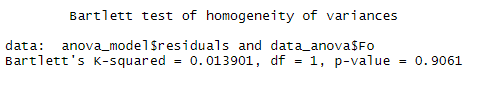
\includegraphics[width=\linewidth]{anova_homo}
	\end{center}
	\caption{Prueba de Bartlett \label{fig:anova_homo}}%
\end{figure}

\section{Clústeres}\label{sec:clusters}

En el siguiente análisis utilizando clústeres se tomó como referencia los resultados obtenidos del análisis de las componentes principales, en las que según el críterio del porcentaje el resultado era dos componentes principales y según el críterio de Kaiser el resultado era tres componentes principales.

\begin{figure}[htb]%
	\begin{center}
		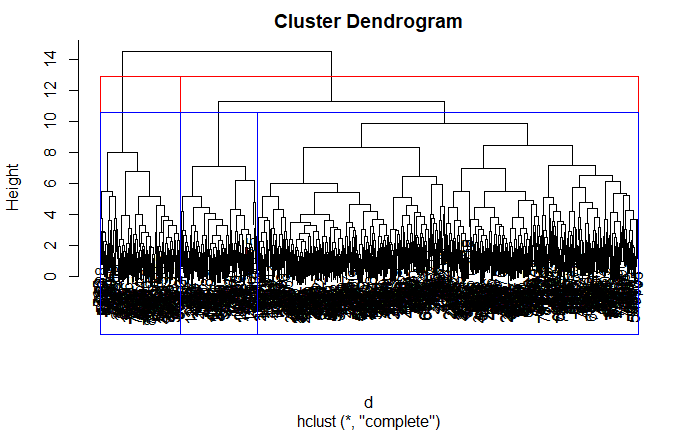
\includegraphics[width=\linewidth]{dendogram_2_3}
	\end{center}
	\caption{Dendograma con 2 y 3 clústeres \label{fig:dendogram_2_3}}%
\end{figure}

Analizando los dendrogramas (Fig. \ref{fig:dendogram_2_3}) se puede observar que tanto para $2$ como para $3$ clústeres existe uno de los clústeres que tiene la mayoría de los datos, por lo que se analizó aumentar la cantidad de clústeres a $4$, $5$, $6$ y $7$ para analizar el comportamiento con estas cantidades.

\begin{figure}[htb]%
	\begin{center}
		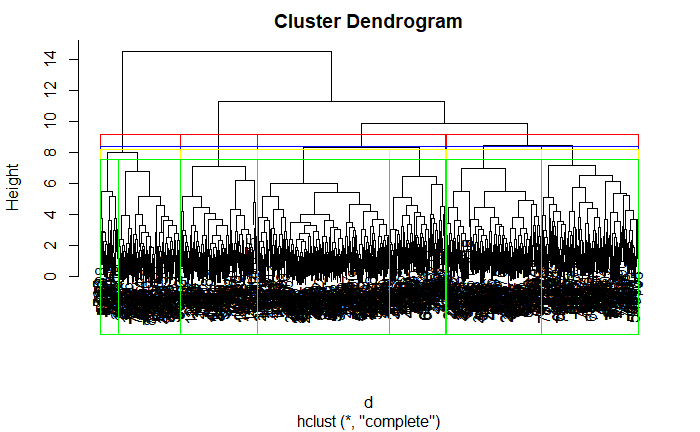
\includegraphics[width=\linewidth]{dendogram_4_7}
	\end{center}
	\caption{Dendograma con 4, 5, 6 y 7 clústeres \label{fig:dendogram_4_7}}%
\end{figure}

Del análisis del dendograma (Fig. \ref{fig:dendogram_4_7}) se eligió $6$ clústeres como medidor principal debido a que con $4$ y $5$ clústeres permanecía una diferencia sustancial en cuanto a la cantidad de datos en cada clúster, y con $7$ clústeres no se observó una mejora sobre a elección de $6$ clústeres. Tomando en cuenta que se están segmentando en grupos a jugadores de futbol según sus características, $6$ grupos no es una división exagerada, ya que los jugadores se pueden dividir por posiciones en el campo, estilo: portero, defensas centrales, laterales, medio campistas defensivos, medio campistas ofencivos y delanteros. No quiere decir que el análisis con $6$ clústeres determine estos grupos, solamente se quisó ilustrar que una clasificación en $6$ grupos a los futbolistas no es una división extraña.

\section{K-Medias}\label{sec:kmeans}

Se realizó un análisis utilizando el algoritmo de K-medias. Se utilizaron $6$ particiones basándose en el resultado del análisis de los clústeres.

\begin{figure}[htb]%
	\begin{center}
		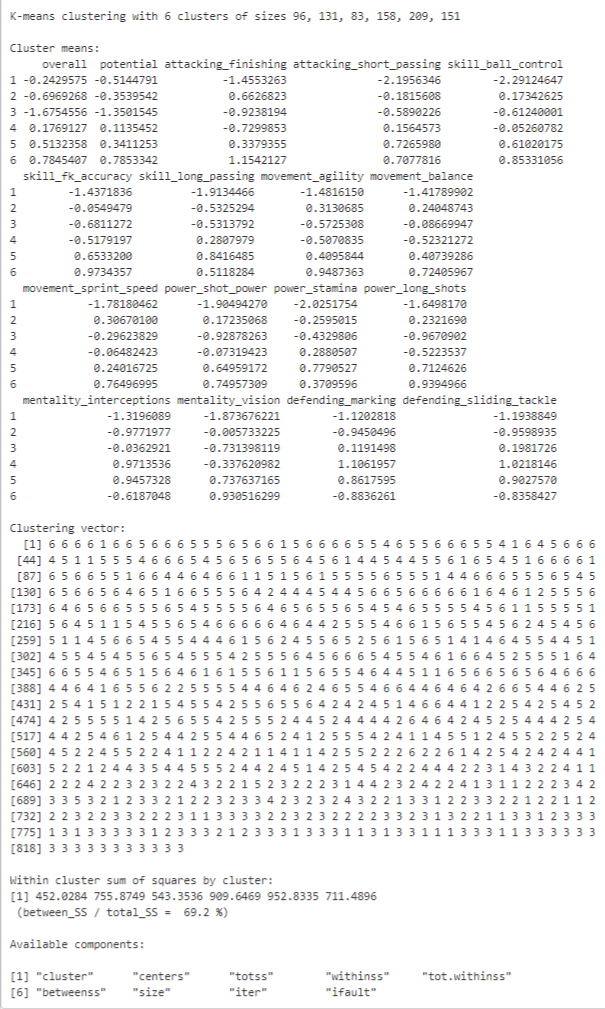
\includegraphics[width=\linewidth]{kmeans}
	\end{center}
	\caption{Resultado de K-medias \label{fig:kmeans}}%
\end{figure}

Del análisis de los resultado de K-medias (Fig. \ref{fig:kmeans}) se obtuvo que el porciento de similitud es del $69\%$ aproximadamente, lo cual es bastante bueno para la naturaleza de los datos que se analizaron. La cantidad de elementos en cada partición fue de $94$, $168$, $207$, $98$, $122$, $139$ respectivamente.

\section{Árbol de Decisión}\label{sec:dtree}

En un inicio, debido a que el modelo de regresión lineal no fue útil, ya que se incumplieron sus supuestos, se decidió realzar un análisis utilizando árboles de decisión, en primer árbol de decisión se realizó utilizando las $17$ variables seleccionadas y como variable respuesta a $overall$, el resultado se puede observar en la Fig. \ref{fig:dtree}, pero el error es del $99\%$ por lo que se intento con un segundo árbol de decisión utilizando como variable respuesta $mentality\_interceptions$ y como variables independientes a las componentes principales, nuevamente el error fue alto, cercano al $98\%$. (Fig. \ref{fig:dtree2})

\begin{figure}[htb]%
	\begin{center}
		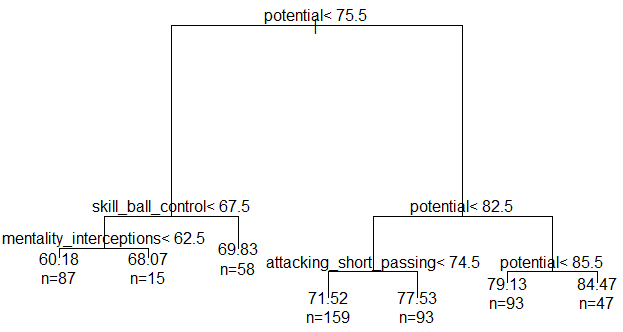
\includegraphics[width=\linewidth]{dtree}
	\end{center}
	\caption{Árbol de Decisión con $overall$ \label{fig:dtree}}%
\end{figure}

\begin{figure}[htb]%
	\begin{center}
		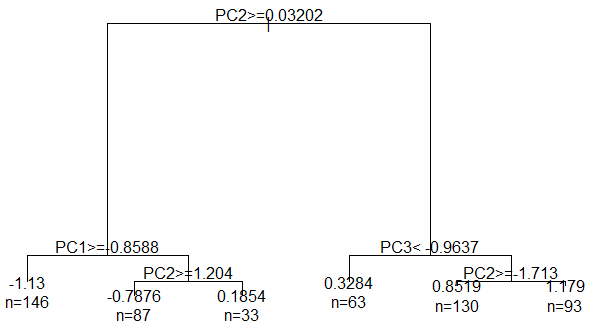
\includegraphics[width=\linewidth]{dtree2}
	\end{center}
	\caption{Árbol de Decisión con $mentality\_interceptions$ \label{fig:dtree2}}%
\end{figure}

\section{Conclusiones}\label{sec:conc}

Se realizó un análisis sobre los datos obtenidos, aplicando una regresión lineal junto a un análisis de componente principales, además de un análisis de varianza o ANOVA. En ambos casos, los supuestos de los modelos se incumplieron, pero se pudo mostrar la aplicación de las principales técnicas de regresión y análisis de varianzas para un uso posterior en otras circunstancias y/o datos.

\section{Referencias}\label{sec:ref}

\begin{itemize}
	\item Conferencia 5 - Correlación
	\item Conferencia 6 - Regresión Lineal Simple
	\item Conferencia 7 - Regresión Lineal Múltiple
	\item Conferencia 8 - ANOVA
	\item Conferencia 9 - ACP
	\item Conferencia 10 - Clúster, Árboles de Decisión
\end{itemize}

\label{end}

\end{document}

%===================================================================================
